\documentclass[letterpaper,11pt]{article}

\usepackage{amsmath,amssymb,amsthm}
\usepackage[margin=2.0cm]{geometry}
\usepackage{float}
\usepackage{tikz}

\usetikzlibrary{arrows,automata}

\author{Jacob Thomas Errington (260636023)}
\title{Assignment \#2 \\ Theory of Computation -- COMP 330}
\date{8 October 2015}

\begin{document}

\maketitle

\begin{enumerate}
    \item
        Give regular expressions for the following languages over $\{a, b\}$.

        \begin{enumerate}
            \item $\{w | w \text{ begins and ends with } a\}$

                $$
                a(a + b)^*a + a
                $$

            \item $\{w | \text{ every odd position in $w$ is a } b\}$

                $$
                (b(a + b))^*(b + \epsilon)
                $$

            \item
                $\{w | w \text{ contains at least two $a$s and at most one $b$}\}$

                $$
                a^*aaa^*(b+\epsilon)a^* +
                a^*(b+\epsilon)a^*aaa^* +
                a^*a(b+\epsilon)aa^*
                $$
        \end{enumerate}

    \item
        Give NFAs for the following regular expressions.

        \begin{enumerate}
            \item
                $\epsilon + a(a + b)^* + (a + b)^*aa(a + b)^*$

                \begin{figure}[H]
                    \centering

                    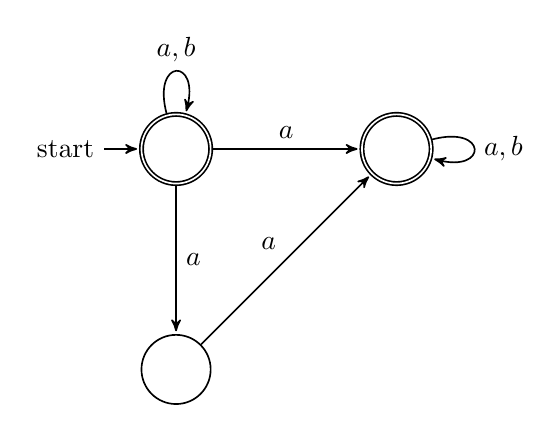
\begin{tikzpicture}[
                            ->,
                            >=stealth',
                            shorten >=1pt,
                            auto,
                            node distance=2.8cm,
                            semithick
                        ]
                        \tikzstyle{every state}=[fill=white,draw=black,text=black]

                        \node[initial,accepting,state] (A) {} ;
                        \node[state,accepting]         (B) [right of=A] {};
                        \node[state]                   (D) [below of=A] {};

                        \path
                        (A) edge [loop above]  node {$a,b$} (A)
                        (A) edge               node {$a$}   (B)
                        (B) edge [loop right]  node {$a,b$} (B)
                        (D) edge               node {$a$}   (B)
                        (A) edge               node {$a$}   (D)
                        ;
                    \end{tikzpicture}
                \end{figure}

            \item
                $\left[ ba + (a + bb)a^*b \right]^*$

                \begin{figure}[H]
                    \centering

                    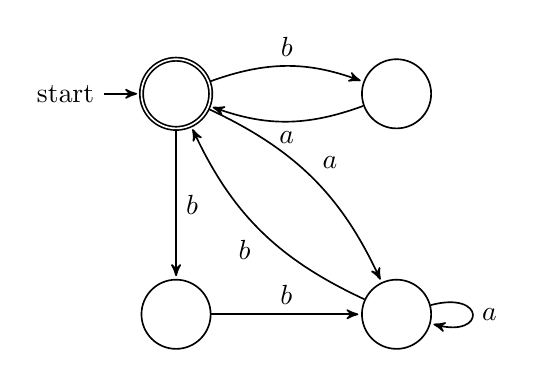
\begin{tikzpicture}[
                            ->,
                            >=stealth',
                            shorten >=1pt,
                            auto,
                            node distance=2.8cm,
                            semithick
                        ]
                        \tikzstyle{every state}=[fill=white,draw=black,text=black]

                        \node[initial,accepting,state] (A) {} ;
                        \node[state]                   (B) [right of=A] {} ;
                        \node[state]                   (C) [below of=A] {} ;
                        \node[state]                   (D) [right of=C] {} ;

                        \path
                        (A) edge [bend left=20]  node {$b$} (B)
                        (B) edge [bend left=20]  node {$a$} (A)
                        (A) edge                 node {$b$} (C)
                        (C) edge                 node {$b$} (D)
                        (A) edge [bend left=20]  node {$a$} (D)
                        (D) edge [loop right]    node {$a$} (D)
                        (D) edge [bend left=20]  node {$b$} (A)
                        ;
                    \end{tikzpicture}
                \end{figure}
        \end{enumerate}

    \item Show that the following languages are regular over the alphabet
        $\{a, b\}$.

        \begin{enumerate}
            \item
                $\{xwx^R | x \in \Sigma^*, w \in \Sigma^*, |x| > 0, |w| > 0\}$
                where $x^R$ means $x$ reversed.

                $$
                a(a+b)^*a + b(a+b)^*b
                $$

            \item
                $\{a^n b^m | n > 0, m > 0, n - m = 0 \mod{3}\}$

                The number of $a$s must match the number of $b$s on their
                remainder in division by three.

                \begin{figure}[H]
                    \centering

                    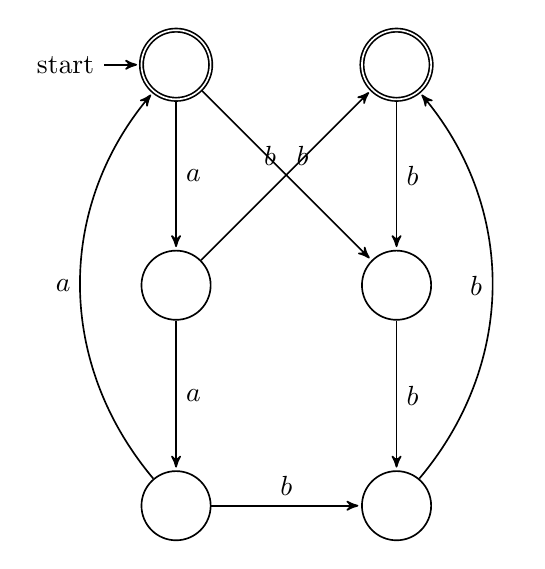
\begin{tikzpicture}[
                            ->,
                            >=stealth',
                            shorten >=1pt,
                            auto,
                            node distance=2.8cm,
                            semithick
                        ]
                        \tikzstyle{every state}=[fill=white,draw=black,text=black]

                        \node[initial,accepting,state] (A) {};
                        \node[state]                   (B) [below of=A] {};
                        \node[state]                   (C) [below of=B] {};
                        \node[accepting,state]         (D) [right of=A] {};
                        \node[state]                   (E) [below of=D] {};
                        \node[state]                   (F) [below of=E] {};

                        \path
                        (A) edge                 node {$a$} (B)
                        (A) edge                 node {$b$} (E)
                        (B) edge                 node {$a$} (C)
                        (B) edge                 node {$b$} (D)
                        (C) edge [bend left=40]  node {$a$} (A)
                        (C) edge                 node {$b$} (F)
                        (D) edge                 node {$b$} (E)
                        (E) edge                 node {$b$} (F)
                        (F) edge [bend right=40] node {$b$} (D)
                        ;
                    \end{tikzpicture}
                \end{figure}

            \item
                $\{a^n b^m | n > 0, m > 0, n + m = 0 \mod 3\}$

                The automaton identified by this regular expression must
                consume some number of $a$s followed by some number of $b$s
                such that the sum of the consumed characters is a multiple of
                three.

                The proposed automaton counts the number of $a$s it consumes,
                mod three. Let $n$ be that number. Upon encountering a $b$, it
                switches to the state corresponding to the count $n$ in a
                second counter, but this time for $b$s.
        \end{enumerate}

    \item The table of inequivalent states is the following.

        \begin{tabular}{c c c}
            A & 0 & A \\
            A & 1 & B \\
            B & 0 & B \\
            B & 1 & A
        \end{tabular}

        The minimal automaton is the following.

        \begin{figure}[H]
            \centering

            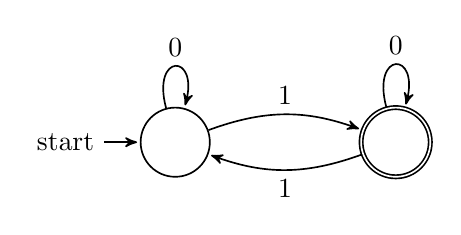
\begin{tikzpicture}[
                    ->,
                    >=stealth',
                    shorten >=1pt,
                    auto,
                    node distance=2.8cm,
                    semithick
                ]
                \tikzstyle{every state}=[fill=white,draw=black,text=black]

                \node[initial,state]    (A) {};
                \node[accepting,state]  (B) [right of=A] {};

                \path
                (A) edge [loop above]   node {$0$} (A)
                (A) edge [bend left=20] node {$1$} (B)
                (B) edge [loop above]   node {$0$} (B)
                (B) edge [bend left=20] node {$1$} (A)
                ;
            \end{tikzpicture}
        \end{figure}

    \item The bisimulation-minimal LTS is the following.

        \begin{figure}[H]
            \centering

            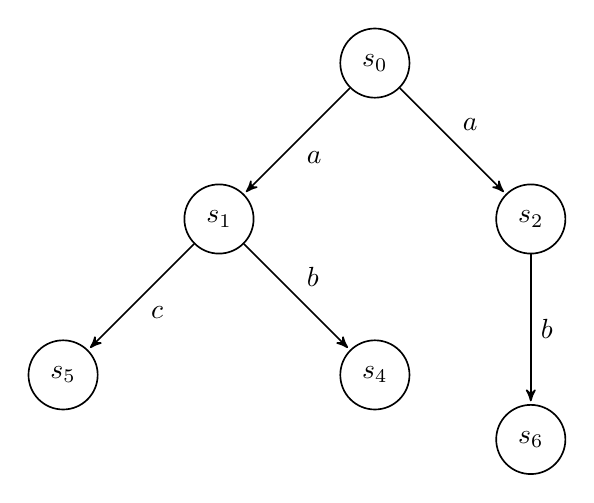
\begin{tikzpicture}[
                    ->,
                    >=stealth',
                    shorten >=1pt,
                    auto,
                    node distance=2.8cm,
                    semithick
                ]
                \tikzstyle{every state}=[fill=white,draw=black,text=black]

                \node[state] (A) {$s_0$};
                \node[state] (B) [below left of=A] {$s_1$} ;
                \node[state] (C) [below right of=A] {$s_2$} ;
                \node[state] (D) [below right of=B] {$s_4$} ;
                \node[state] (E) [below left of=B] {$s_5$} ;
                \node[state] (F) [below of=C] {$s_6$} ;

                \path
                (A) edge node {$a$} (B)
                (A) edge node {$a$} (C)
                (B) edge node {$c$} (E)
                (B) edge node {$b$} (D)
                (C) edge node {$b$} (F)
                ;

            \end{tikzpicture}
        \end{figure}

\end{enumerate}
\end{document}
